\chapter{Discussion and Experiments}
\label{chap:orderbookagents}
This chapter summarizes various experiments, that have been conducted to examine the agents ability to find optimal solutions to the problem of optimized trade execution. The recorded orderbook snapshots for currency pair USDT/BTC (see \Cref{chap:dataorigin}) have been split into training period (Nov, 10th 2016 - Apr, 30th 2017) and test period (May 2017).\\

All experiments refer to the very same environment settings. The agents common task is to buy Bitcoins worth of 70.000\$ within a trading horizon of 60 minutes. The problem definition is opposed to the task evaluated by Nevmyvaka \etal \cite{Nevmyvaka:2006}, where the number of shares (respectively Bitcoins) was fixed, rather than the amount of cash.\\

The training set translates into 4.154 orderbook windows, while the test set gives 724 orderbook windows. A period length of 15 minutes is assumed, such that the \ac{OTS} expects up to $T=4$ order limit prices. Private variable \lstinline!volume! is discretized in 8 intervals, \ie $I=[8.750\$,..,70.000\$]$, and the action space consists of fifteen actions $L=[-4, -3, ..., 8, 9, 10]$. In line with the formulas presented in \Cref{chap:actionspace}, these actions translate into order limits deviating by $-0.4\%$ to $+1.0\%$ from the current best price.


\subsection{Baseline}
\label{chap:experiments:baseline}
Simple \ac{SL} strategies (see \Cref{chap:tradingstrategies}) and immediate market order placements serve as benchmark for the performance measurement.\\

\begin{figure}[ht]
	\centering
	\begin{subfigure}[b]{0.5\textwidth}
        		\centering
        		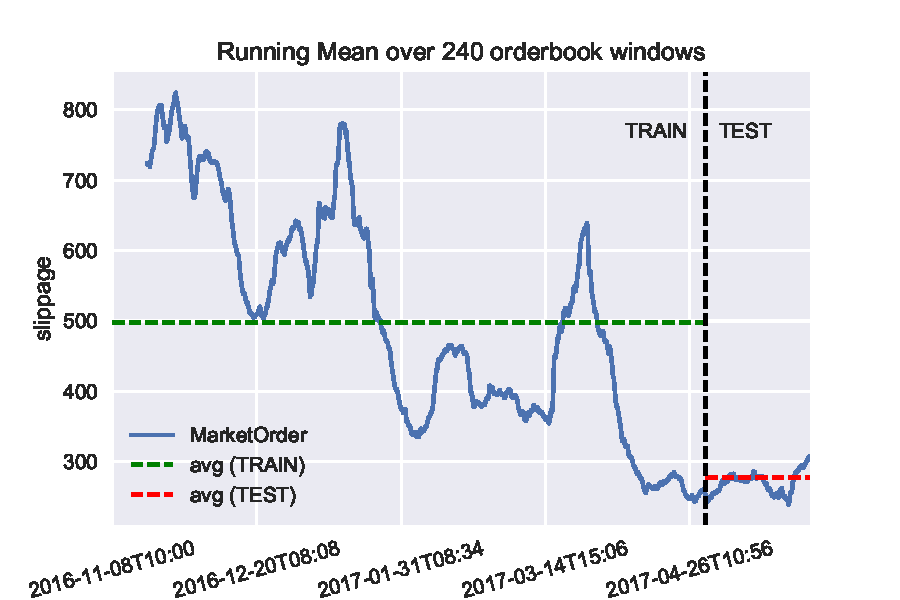
\includegraphics[width=\textwidth]{content/drawings/runningMean240_MarketPrice}
        		\caption{Observed Market Order Slippage.}
		\label{fig:runningmean:marketPrice}
    	\end{subfigure}%
	\begin{subfigure}[b]{0.5\textwidth}
        		\centering
        		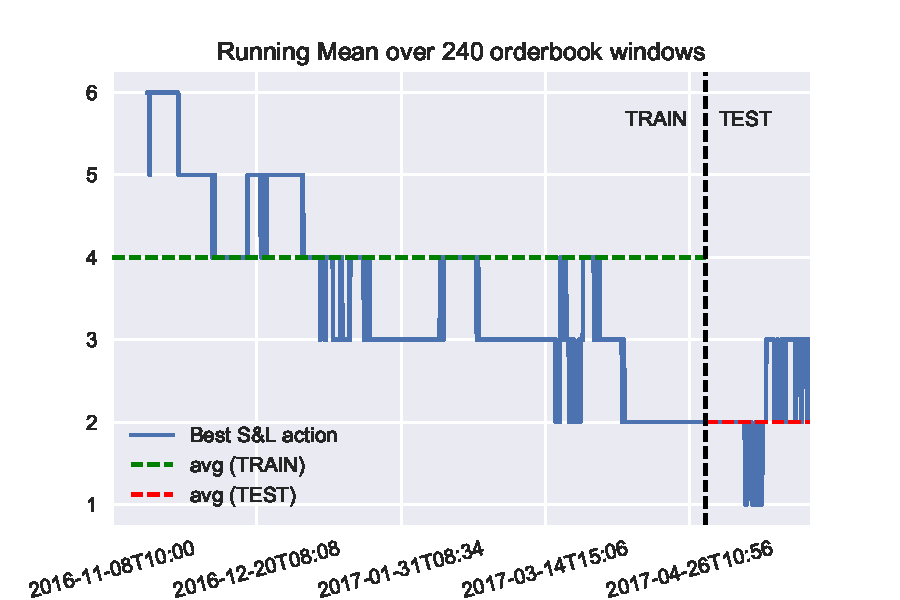
\includegraphics[width=\textwidth]{content/drawings/runningMean240_bestAction}
        		\caption{Best S\&L action.}
		\label{fig:runningmean:bestaction}
    	\end{subfigure}

	\caption{Concurrent to declining slippage, the optimal \ac{SL} actions become less aggressive as time passes.}
	\label{fig:runningmean}
\end{figure}


\begin{figure}[ht]
        	\centering
        	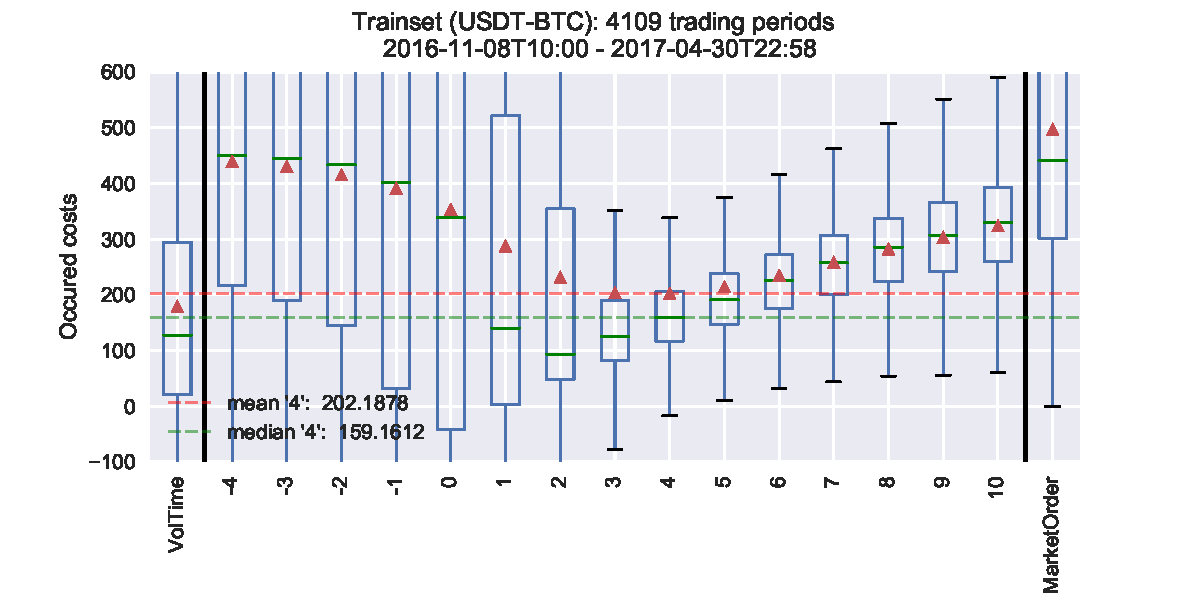
\includegraphics[width=\textwidth]{content/drawings/bestActionTrain}
	\caption{Average costs induced by the varying \ac{SL} actions over the full training period. In average, action 4 performed best.}
	\label{fig:bestAction}
\end{figure}

Due to bursting Bitcoin prices (see \Cref{chap:dataorigin}, \Cref{fig:ploniexPriceHistory}), the investigated sum of 70.000\$ constitutes a declining contingent of the total market volume. \Cref{fig:runningmean:marketPrice} shows a running average over the amount of slippage, as induced by immediate market orders. Concurrent to declining slippage, the optimal \ac{SL} actions become less aggressive as time passes. The green, dashed lines show the respective average over the training period, which significantly differs from the red, dotted line referring to the average over the test period. \Cref{fig:bestAction} shows the average costs, induced by varying \ac{SL} strategies within the training period.\\

In order to provide a more realistic and unexaggerated baseline, the optimal \ac{SL} action is estimated from the test period. As such, performance of subsequents experiments are compared to the performance of a simple market order and the \ac{SL} strategy "2", with the initial order limit fixed to 1.002 times the initial ask (\ie $+0.2\%$).


\section{Examined Issues}
\label{chap:backwardalgorithm:discussion}
While the presented backward algorithm exploits the available data profoundly in a brute force manner, the underlying assumptions deserve a short discussion. Alternative formulations are tested out, to potentially improve the algorithms cost saving capabilities.

\subsection{Action-Limit Mapping}
\label{chap:backwardalgorithm:discussion:actionspace}
By fixing the limit base at the best price of the \emph{opposing} book, it appears obvious, that decisions derived from state spaces including a variable for the current spread size, outperform decisions derived from state spaces not including this market variable. Indeed, in the original paper\Cite{Nevmyvaka:2006} the bid-ask spread was posed as the market variable causing the greatest individual impact on cost reduction, namely -$7.97\%$, which is a major fraction of the maximum achievement of  $-12.85\%$\footnote{Strategies derived from five dimensional state spaces including the market variables Spread, ImmCost \& Signed Vol, as described in \Cref{chap:costs}, outperformed strategies derived from two dimensional state spaces, containing the private variables only, by $-12.85\%$ in average.}.\\

The influence of moving the limit base to the opposite book, as proposed in \Cref{chap:actionspace}, is analyzed in \Cref{chap:exp:actionlimitmapping}.


\subsection{Discrete State Space}
The most obvious weakness of the discrete backward approach lies in its vulnerability to seldomly observed market situations. Since the state-action function is implemented as a simple lookup table without any generalization capabilities, it is strictly dependent on a thorough exploration of the underlying state space. As exhaustive exploration is enforced for the value range of private variables only, market variables are entrusted to chance. Especially when increasing the state space dimension by adding multiple market variables simultaneously, the explanatory power of a learned state-action mapping depends crucially on the number of underlying observations. There exists even the chance of certain states never been monitored at all during the training phase.\\

Consequently, the impact of different market variables at varying levels of discretization is examined, starting in \Cref{chap:exp:additionalmarketvars}. Eventually, the effect of replacing the underlying lookup table with function approximators is studied in \Cref{chap:experiment:functionApprox}. 





\subsection{Markov Property}
\label{chap:backwardalgorithm:discussion:markovianassumption}
The proposed backward algorithm (see \Cref{chap:backwardlearning}, \Cref{alg:bruteforce:pseudocode}) assumes individual \lstinline!trading_periods! to be of an (approximately) Markovian nature. As explained in \Cref{chap:backwardapproach:precedingTrades}, the \ac{OTS}'s internal masterbook shape depends drastically from the preceding trade history. Since all relevant information from the history must be taken into account, two approaches are examined, that aim to generate more realistic samples and as such to strengthen the Markov Property of states:\\

The advantage of the improved backward algorithm, that takes preceding trades into account (see \Cref{chap:backwardapproach:precedingTrades}, \Cref{alg:bruteforceimproved:pseudocode}), is shown in \Cref{chap:exp:simulatedTrades}. \Cref{chap:experiments:forward} demonstrates, that the novel forward sampling algorithm described in \Cref{chap:forwardlearning} outperforms all other methods, as strategies are derived from a more realistic set of sample transitions.

% than that, a more realistic sampling method may be applied: The forward sampling process, described in \Cref{chap:forwardlearning}, approaches sampling from the other side. Rather than evaluating actions on individual \lstinline!trading_periods!, the \ac{OTS} always starts with $V=100 \% $ and keeps going until the full trade is executed. As such, more realistic samples are generated. This does not give the problem a Markovian nature, but the internal masterbook is always of a realistic shape. In contrast to the backward approach, exhaustive exploration of the state space is not self-evident and must be enforced.
%As a side benefit, the forward sampling approach generates more versatile samples for training the function approximates, as the generated samples do not necessarily start at \emph{discrete} start points only.







\section{Backward Learning Experiments}
\label{chap:experiments}
In the following, backward learning experiments that paved the way towards improved trade execution strategies are presented.

\subsection{Action-Limit Mapping}
\label{chap:exp:actionlimitmapping}
As mentioned in \Cref{chap:backwardalgorithm:discussion:actionspace}, it seems pointless to force actions to cross the bid-ask-spread before any orders can be matched. \Cref{fig:actionlimitmapping} shows exemplary for November 2016, how the choice of the limit base affects the agents trading performance.\\

\begin{table}[ht]
	\centering
		\scalebox{0.7}{
\rowcolors{1}{}{black!5}
\begin{tabular}{|lRR|}
\toprule
{} &           slippage & performance \\
\midrule
currBid         	     &  220.19 & 92.6\%\\
currBid\_mSpread &  218.71 & 91.9\%\\
currBid\_spread     &  215.76 & 90.7\%\\
\midrule
currAsk                  &  214.00 & 90.0\%\\
currAsk\_mSpread &  214.53 &90.2\%\\
currAsk\_spread    &  215.38 & 90.6\%\\
\midrule
S\&L: 5         	      & 237.75 & 100.0\%\\
MarketOrder          & 737.58 & 310.2\%\\
\bottomrule
\end{tabular}	
		} 
	\caption{Evaluating the impact of different limit base levels.}
	\small Results stem from applying the respective strategies on all 537 orderbook\\ windows recorded between Nov, 10th 2016 and Nov, 30th 2016.
	\label{fig:actionlimitmapping}
\end{table}

While buy orders, forcing agents to cross the bid-ask-spread (\ie \lstinline!currBid*!), typically benefit from the two market variables \lstinline!spread! and \lstinline!marketSpread!, this is not necessarily the case for agents which have the limit base fixed to the opposing best price (\ie \lstinline!currAsk*!). As the latter agents consistently showed better performance, the limit base is henceforth fixed to the best price of the corresponding trading direction.





\subsection{Additional Market Variables}
\label{chap:exp:additionalmarketvars}
In addition to the originally proposed market variables (see \Cref{chap:statespace}), the following orderbook features have been examined:

\begin{description}
\item[marketPrice*] describes the relative difference between current center price and the worst price that must be paid (or is received) in case of simple market orders.

\item[sharecount\_*] quotes the number of Bitcoins, immediately available for $70.000\$$.\\
\lstinline!sharecount_buy! is tantamount to the originally proposed \lstinline!ImmCost! (See \Cref{chap:backwardalgorithm:discussion:subjectTrade}).

\item[center\_price] was added as a consequence of the findings from \Cref{chap:experiments:baseline}, \Cref{fig:runningmean}: Apparently, as the ratio between current Bitcoin price and the investable $70.000\$$ increases, an optimal strategy may have to place less aggressive order limits.

\item[\_a*\_effects] quotes the minimum volume immediately obtainable by individual actions. The value is a lower bound of the truly obtainable volume, because only the current orderbook is retrievable. New opportunities, arising within the forthcoming \lstinline!trading_period! are unacquainted and not included.
\end{description}


 \Cref{tab:eval:additionalMarketVariables} shows the performance of individual QTable agents trained on both private variables plus one discretized market variable attached at a time. While observed trading costs undercut those induced by simple market orders by $-49.16\%$, the gain in comparison to the optimal \ac{SL} strategy lies at $-8.93\%$.\\
 
Adding the market variable \lstinline!spread! yields a notable improvement of $-4.84\%$ over the plain \lstinline!VolTime!-agent. By increasing the discretization level to 5, the performance can be further improved to $-6.34\%$, verifying the findings of Nevmyvaka�\etal \Cite{Nevmyvaka:2006}. However, in contrast to their reported results, the market variable \lstinline!sharecount_buy! falls flat with a worsening of $+6.70\%$ (compared to $-4.26\%$).\\
 
Disappointing is the futility of \lstinline!center_price!. For a discretization level of 5, the corresponding agent underperforms the plain \lstinline!VolTime!-agent by $+7.35\%$. Potentially, this may be explained by a compulsorily underexploited training set: Due to generally rising Bitcoin prices, the majority of prices in the test period will map to the highest discretization value available, which, in a simple lookup-table, resembles only a fraction of the assessed training set.\\

\begin{table}[ht]
	\centering
	\scalebox{0.6}{
	\rowcolors{1}{}{black!5}
\begin{tabular}{|lRRR|RRRR|}
\toprule
{} &  \text{slippage} &     \text{med} &     \text{std} &   \text{perf\_2} &   \text{perf\_4} &   \text{perf\_M} & \text{perf\_VolTime} \\
\midrule
center\_price\_disc3            &    149.57 &   46.15 &  420.14 &   -3.44\% &  -15.19\% &  -46.10\% &       -0.70\% \\
center\_price\_disc5            &    161.70 &   37.83 &  450.36 &    +4.39\% &   -8.32\% &  -41.73\% &        \cellcolor{red!25}+7.35\% \\
marketPrice\_buy\_worst\_disc5  &    146.83 &   39.62 &  351.77 &   -5.21\% &  -16.75\% &  -47.08\% &       -2.52\% \\
marketPrice\_sell\_worst\_disc5 &    148.94 &   42.71 &  388.86 &   -3.85\% &  -15.55\% &  -46.33\% &       -1.12\% \\
marketPrice\_spread\_disc5     &    150.46 &   44.15 &  371.32 &   -2.87\% &  -14.69\% &  -45.78\% &       -0.11\% \\
marketPrice\_imbalance\_disc5      &    150.10 &   68.68 &  336.60 &   -3.10\% &  -14.90\% &  -45.91\% &       -0.35\% \\
sharecount\_buy\_disc3         &    149.57 &   46.15 &  420.14 &   -3.44\% &  -15.19\% &  -46.10\% &       -0.70\% \\
sharecount\_buy\_disc5         &    160.73 &   37.78 &  449.22 &    +3.76\% &   -8.87\% &  -42.08\% &        \cellcolor{red!25}+6.70\% \\
sharecount\_imbalance\_disc5   &    148.03 &   40.49 &  372.86 &   -4.44\% &  -16.07\% &  -46.65\% &       -1.73\% \\
sharecount\_sell\_disc5        &    151.50 &   47.49 &  425.35 &   -2.20\% &  -14.10\% &  -45.40\% &        +0.58\% \\
sharecount\_spread\_disc5      &    148.93 &   40.84 &  352.12 &   -3.86\% &  -15.56\% &  -46.33\% &       -1.13\% \\
spread\_disc3                 &    147.41 &   35.48 &  370.96 &   \cellcolor{black!20}-4.84\% &  -16.42\% &  -46.88\% &       -2.14\% \\
spread\_disc5                 &    \cellcolor{green!25}141.07 &   \cellcolor{green!25}37.39 &  \cellcolor{green!25}349.72 &   \cellcolor{green!25}-8.93\% &  \cellcolor{green!25}-20.02\% &  \cellcolor{green!25}-49.16\% &       \cellcolor{green!25}-6.34\% \\
spread\_disc9                 &    142.80 &   36.69 &  364.76 &   -7.81\% &  -19.03\% &  -48.54\% &       -5.20\% \\
\midrule
VolTime                      &    150.63 &   33.83 &  358.66 &   -2.76\% &  -14.60\% &  -45.72\% &        0.00\% \\
2                            &    154.90 &   68.62 &  389.15 &    0.00\% &  -12.17\% &  -44.18\% &        +2.84\% \\
4                            &    176.37 &  141.66 &  273.58 &   +13.86\% &    0.00\% &  -36.44\% &       +17.09\% \\
MarketOrder                  &    277.49 &  246.48 &  158.66 &   +79.14\% &   +57.33\% &    0.00\% &       +84.22\% \\
\bottomrule
\end{tabular}
	}  		 
        		\caption{Evaluating the impact of additional market variables.}
		\small Average performance over the test period may 2017, currency pair USDT/BTC.\\
		See \Cref{appendix:additionalMarketVariables}, \Cref{tab:eval:additionalMarketVariables:fulltable} for complete results.
		\label{tab:eval:additionalMarketVariables}

\end{table}

The different discretization levels yield rather mixed results. While \lstinline!spread! typically performed best in case of 5 levels, no clear statement can be made for the other variables.\\

The exact reason, why factually only adding \lstinline!spread! causes a beneficial effect, is unclear, but one possible explanations lies in the data set employed. The original experiment assessed a different data quality. Due to the low resolution of the available orderbook snapshots, a large fraction of the market activity remains inaccessible and consequently the majority of trading opportunities are missed by the agents. Furthermore, the minute time-scaled data inevitably requires the trading horizon to be rather long. Experiments with shorter time horizons nullified the achievable savings, while longer time horizons led to unacceptable computation times. Consequently, the agents where trained on $4.109$ sixty-minute orderbook windows, while Nevmyvaka \etal invoked $45.000$ two-minute orderbook windows.


\subsection*{Look-Ahead Features}
\label{chap:experiments:lookahead}
In order to proof the algorithms general ability to find costs reducing strategies, look-ahead features\footnote{look-ahead features provide a glance into the future, and are thus equivalent to cheating.} were added to the universe of market variables. \lstinline!future_center*! quotes percentual changes between the current center price and the center price in 5, 15 and 60 minutes respectively. This hypothetical knowledge about future price trends reduces observed trading costs by $-12.47\%$ (\ie $-14.88\%$ over simple \ac{SL} strategy).\\

\begin{table}[ht]
	\centering
	\scalebox{0.6}{
	\rowcolors{1}{}{black!5}
\begin{tabular}{|lRRR|RRRR|}
\toprule
{} &  \text{slippage} &     \text{med} &     \text{std} &   \text{perf\_2} &   \text{perf\_4} &   \text{perf\_M} & \text{perf\_VolTime} \\
\midrule
ob\_direction\_disc5           &     61.99 &   97.52 &  319.84 &  \cellcolor{black!20}-59.98\% &  -64.85\% &  -77.66\% &      \cellcolor{black!20}-58.84\% \\
future\_center5\_disc5         &    141.61 &   41.79 &  389.58 &   -8.58\% &  -19.71\% &  -48.97\% &       -5.98\% \\
future\_center15\_disc5        &    133.78 &   40.90 &  405.88 &  -13.63\% &  -24.15\% &  -51.79\% &      -11.18\% \\
future\_center60\_disc5        &    131.85 &   47.63 &  391.46 &  \cellcolor{green!25}-14.88\% &  -25.25\% &  -52.49\% &      \cellcolor{green!25}-12.47\% \\
\midrule
VolTime                      &    150.63 &   33.83 &  358.66 &   -2.76\% &  -14.60\% &  -45.72\% &        0.00\% \\
2                            &    154.90 &   68.62 &  389.15 &    0.00\% &  -12.17\% &  -44.18\% &        +2.84\% \\
4                            &    176.37 &  141.66 &  273.58 &   +13.86\% &    0.00\% &  -36.44\% &       +17.09\% \\
MarketOrder                  &    277.49 &  246.48 &  158.66 &   +79.14\% &   +57.33\% &    0.00\% &       +84.22\% \\
\bottomrule
\end{tabular}
	}  		 
        		\caption{Evaluating the impact of look-ahead features.}
		\small Average performance over the test period may 2017, currency pair USDT/BTC.\\
		\label{tab:eval:additionalMarketVariables:lookahead}

\end{table}

A vastly larger impact ($-58.84\%$ respectively $-59.98\%$) is caused by the look-ahead feature \lstinline!ob_direction!, quoting the general price trend of the currently observed orderbook window. In contrast to the \lstinline!future_center*! variables, it's value stays constant within individual orderbook windows: \lstinline!ob_direction = orderbook[-1].get_center() / orderbook[0].get_center()!, which seems to provoke more stable strategies.


\subsection*{Constant Market Variables}
\label{chap:exp:additionalmarketvars:constant}
The findings from the look-ahead features encouraged for a supplementary experiment. Rather than considering the actual market situation, the market variables are observed once (at \lstinline!t=0!), and kept frozen for the remaining trading horizon. Hope was, to provoke more stable strategies, as the agents could potentially decide on a \emph{major} strategy and consequently only adapt the limits to the private variables representing the actual trade progress.\\

\begin{table}[ht]
	\centering
	\scalebox{0.6}{
	\rowcolors{1}{}{black!5}
\begin{tabular}{|lRRR|RRRR|}
\toprule
{} &  \text{slippage} &     \text{med} &     \text{std} &   \text{perf\_2} &   \text{perf\_4} &   \text{perf\_M} & \text{perf\_VolTime} \\
\midrule
center\_orig\_disc3            &    158.96 &   48.93 &  431.17 &    2.62\% &   -9.87\% &  -42.71\% &        +5.54\% \\
center\_orig\_disc5            &    150.37 &   47.01 &  422.14 &   -2.92\% &  -14.74\% &  -45.81\% &       \cellcolor{red!25}-0.17\% \\
marketPrice\_buy\_worst\_disc5  &    150.74 &   50.15 &  402.13 &   -2.69\% &  -14.54\% &  -45.68\% &        +0.07\% \\
marketPrice\_sell\_worst\_disc5 &    157.56 &   43.95 &  379.33 &    +1.72\% &  -10.66\% &  -43.22\% &        +4.61\% \\
marketPrice\_spread\_disc5     &    152.19 &   53.07 &  398.10 &   -1.75\% &  -13.71\% &  -45.15\% &        +1.04\% \\
marketPrice\_imbalance\_disc5      &    147.16 &   47.03 &  383.19 &   -5.00\% &  -16.57\% &  -46.97\% &       \cellcolor{black!20}-2.30\% \\
sharecount\_buy\_disc3         &    149.57 &   46.15 &  420.14 &   -3.44\% &  -15.19\% &  -46.10\% &       -0.70\% \\
sharecount\_buy\_disc5         &    150.37 &   47.01 &  422.14 &   -2.92\% &  -14.74\% &  -45.81\% &       \cellcolor{red!25}-0.17\% \\
sharecount\_imbalance\_disc5   &    152.44 &   53.41 &  400.89 &   -1.59\% &  -13.57\% &  -45.06\% &        +1.20\% \\
sharecount\_sell\_disc5        &    150.37 &   47.01 &  422.14 &   -2.92\% &  -14.74\% &  -45.81\% &       -0.17\% \\
sharecount\_spread\_disc5      &    149.23 &   53.41 &  402.65 &   -3.66\% &  -15.39\% &  -46.22\% &       -0.93\% \\
spread\_disc3                 &    148.92 &   41.70 &  361.12 &   -3.86\% &  -15.57\% &  -46.33\% &       -1.14\% \\
spread\_disc5                 &    \cellcolor{green!25}143.56 &   \cellcolor{green!25}40.78 &  \cellcolor{green!25}350.74 &   \cellcolor{green!25}-7.32\% &  \cellcolor{green!25}-18.60\% &  \cellcolor{green!25}-48.26\% &       \cellcolor{green!25}-4.69\% \\
spread\_disc9                 &    145.54 &   43.25 &  352.05 &   -6.04\% &  -17.48\% &  -47.55\% &       -3.38\% \\
\midrule
VolTime                      &    150.63 &   33.83 &  358.66 &   -2.76\% &  -14.60\% &  -45.72\% &        0.00\% \\
2                            &    154.90 &   68.62 &  389.15 &    0.00\% &  -12.17\% &  -44.18\% &        +2.84\% \\
4                            &    176.37 &  141.66 &  273.58 &   +13.86\% &    0.00\% &  -36.44\% &       +17.09\% \\
MarketOrder                  &    277.49 &  246.48 &  158.66 &   +79.14\% &   +57.33\% &    0.00\% &       +84.22\% \\
\bottomrule
\end{tabular}
	}  		 
        		\caption{Evaluating the impact of constant market variables.}
		\small Average performance over the test period may 2017, currency pair USDT/BTC.\\
		See \Cref{appendix:fixedMarketVars}, \Cref{tab:eval:additionalMarketVariables:fixed:fulltable} for complete results.
		\label{tab:eval:additionalMarketVariables:fixed}

\end{table}

While \Cref{tab:eval:additionalMarketVariables:fixed} shows improved performance for previous bad performers, the leading \lstinline!VolTimeSpread!-agent dropped from $-8.93\%$ to $-7.32\%$. Contrary to initial hopes, this approach did not lead to superior performance and was not further pursued.\\

\subsection{Simulation of preceding trades}
\label{chap:exp:simulatedTrades}
As described in \Cref{chap:backwardalgorithm:discussion:markovianassumption}, the \ac{OTS}'s internal masterbook shape depends drastically from the preceding trade history. In the following, the effect of incorporating the own impact on the market is investigated.\\

\begin{table}[ht]
	\centering
	\scalebox{0.6}{
	\rowcolors{1}{}{black!5}
\begin{tabular}{|lRRR|RRRRR}
\toprule
{} &  \text{slippage} &     \text{med} &     \text{std} &   \text{perf\_2} &   \text{perf\_4} &   \text{perf\_M} & \text{perf\_VolTime} \\
\midrule
center\_orig\_disc3              &    158.97 &   48.93 &  431.16 &    +2.62\% &   -9.87\% &  -42.71\% &        +5.54\% \\
center\_orig\_disc5              &    150.47 &   47.49 &  422.12 &   -2.86\% &  -14.69\% &  -45.78\% &       -0.11\% \\
marketPrice\_buy\_worst\_disc5    &    148.33 &   47.46 &  400.73 &   -4.24\% &  -15.90\% &  -46.55\% &       -1.53\% \\
marketPrice\_sell\_worst\_disc5   &    154.06 &   42.10 &  370.91 &   -0.54\% &  -12.65\% &  -44.48\% &        +2.28\% \\
marketPrice\_spread\_disc5       &    151.12 &   53.07 &  395.68 &   -2.44\% &  -14.32\% &  -45.54\% &        +0.33\% \\
marketPrice\_imbalance\_disc5        &    143.86 &   47.05 &  375.43 &   -7.13\% &  -18.44\% &  -48.16\% &       -4.49\% \\
sharecount\_buy\_disc3           &    149.57 &   46.15 &  420.14 &   -3.44\% &  -15.19\% &  -46.10\% &       -0.70\% \\
sharecount\_buy\_disc5           &    150.47 &   47.49 &  422.12 &   -2.86\% &  -14.69\% &  -45.78\% &       -0.11\% \\
sharecount\_imbalance\_disc5     &    151.92 &   53.41 &  400.69 &   -1.92\% &  -13.86\% &  -45.25\% &        +0.86\% \\
sharecount\_sell\_disc5          &    149.93 &   47.01 &  420.70 &   -3.21\% &  -14.99\% &  -45.97\% &       -0.47\% \\
sharecount\_spread\_disc5        &    149.36 &   53.41 &  402.86 &   -3.58\% &  -15.31\% &  -46.17\% &       -0.84\% \\
spread\_disc3                   &    145.63 &   41.89 &  346.00 &   -5.98\% &  -17.43\% &  -47.52\% &       -3.32\% \\
spread\_disc5                   &    139.87 &   41.22 &  336.30 &   \cellcolor{green!25}-9.70\% &  -20.69\% &  \cellcolor{green!25}-49.59\% &       -7.14\% \\
spread\_disc9                   &    141.30 &   42.80 &  336.88 &   -8.78\% &  -19.89\% &  -49.08\% &       -6.19\% \\
\midrule
ob\_direction\_disc5             &     62.03 &   97.52 &  320.76 &  -59.95\% &  -64.83\% &  -77.64\% &      -58.82\% \\
\midrule
VolTime\_simulatedTrades &    \cellcolor{green!25}147.86 &   \cellcolor{green!25}42.10 &  \cellcolor{green!25}346.17 &   \cellcolor{green!25}-4.55\% &  \cellcolor{green!25}-16.17\% &  \cellcolor{green!25}-46.72\% &       \cellcolor{green!25}-1.84\% \\
VolTime                        &    150.63 &   33.83 &  358.66 &   -2.76\% &  -14.60\% &  -45.72\% &        0.00\% \\
2                              &    154.90 &   68.62 &  389.15 &    0.00\% &  -12.17\% &  -44.18\% &        +2.84\% \\
4                              &    176.37 &  141.66 &  273.58 &   +13.86\% &    0.00\% &  -36.44\% &       +17.09\% \\
MarketOrder                    &    277.49 &  246.48 &  158.66 &   +79.14\% &   +57.33\% &    0.00\% &       +84.22\% \\
\bottomrule
\end{tabular}


\begin{tabular}{||R|}
\toprule
 \text{perf: \Cref{tab:eval:additionalMarketVariables}} \\
\midrule
 -0.70\% \\
 +7.35\% \\
 -2.52\% \\
 -1.12\% \\
 -0.11\% \\
 -0.35\% \\
 -0.70\% \\
 +6.70\% \\
 -1.73\% \\
 +0.58\% \\
 -1.13\% \\
 -2.14\% \\
 -6.34\% \\
 -5.20\% \\
\midrule
-58.84\% \\
\midrule
\\
 \\
 \\
 \\
 \\
\bottomrule
\end{tabular}
}  		 
        		\caption{Evaluating the impact of incorporating preceding trades.}
		\small Average performance over the test period may 2017, currency pair USDT/BTC.\\
		See \Cref{appendix:simPreTrades}, \Cref{tab:eval:additionalMarketVariables:simulatedTrades:fulltable} for complete results.
		\label{tab:eval:additionalMarketVariables:simulatedTrades}

\end{table}

The backward sampling phase is modified, such that prior to the actual trade simulations, the supposedly consumed trading volume is removed from the masterbook. The trading volume affected is matched and removed from the masterbook evenly along the elapsed time, as is indicated in \Cref{chap:backwardapproach:precedingTrades}, \Cref{fig:differingmasterbooks:SimEq}.\\


\Cref{tab:eval:additionalMarketVariables:simulatedTrades} attests a clear improvement over the original sampling method, if preceding trades are incorporated into the \ac{OTS} masterbook. \Cref{fig:heatmap:VolTimeSimpre} shows, how the plain \lstinline!VolTime!-agent becomes slightly more aggressive,  which improves the performance over the optimal \ac{SL} strategy from $-2.76\%$ to $-4.55\%$.\\


\begin{figure}[ht]
	\centering	
	\begin{subfigure}[b]{0.8\textwidth}
        		\centering
        		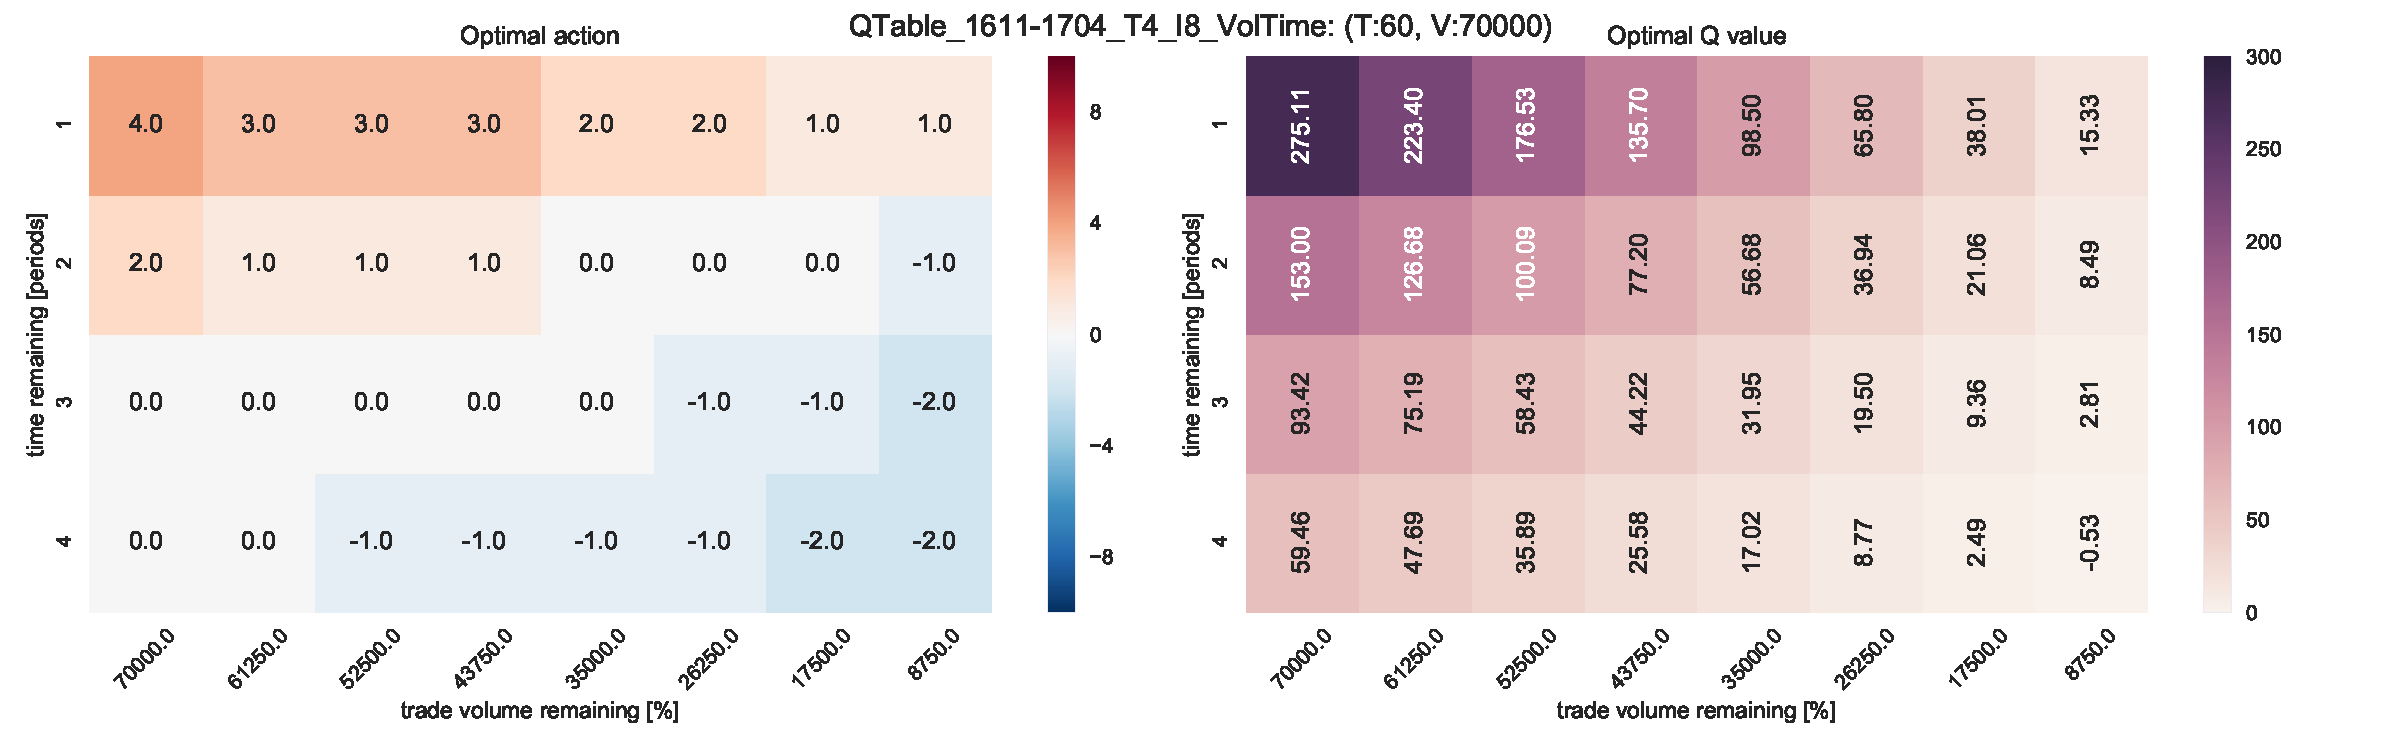
\includegraphics[width=\textwidth]{content/drawings/heatmap_VolTime}
        		\caption{QTable of \lstinline!VolTime!-agent.}
    	\end{subfigure}
	\begin{subfigure}[b]{0.8\textwidth}
        		\centering
        		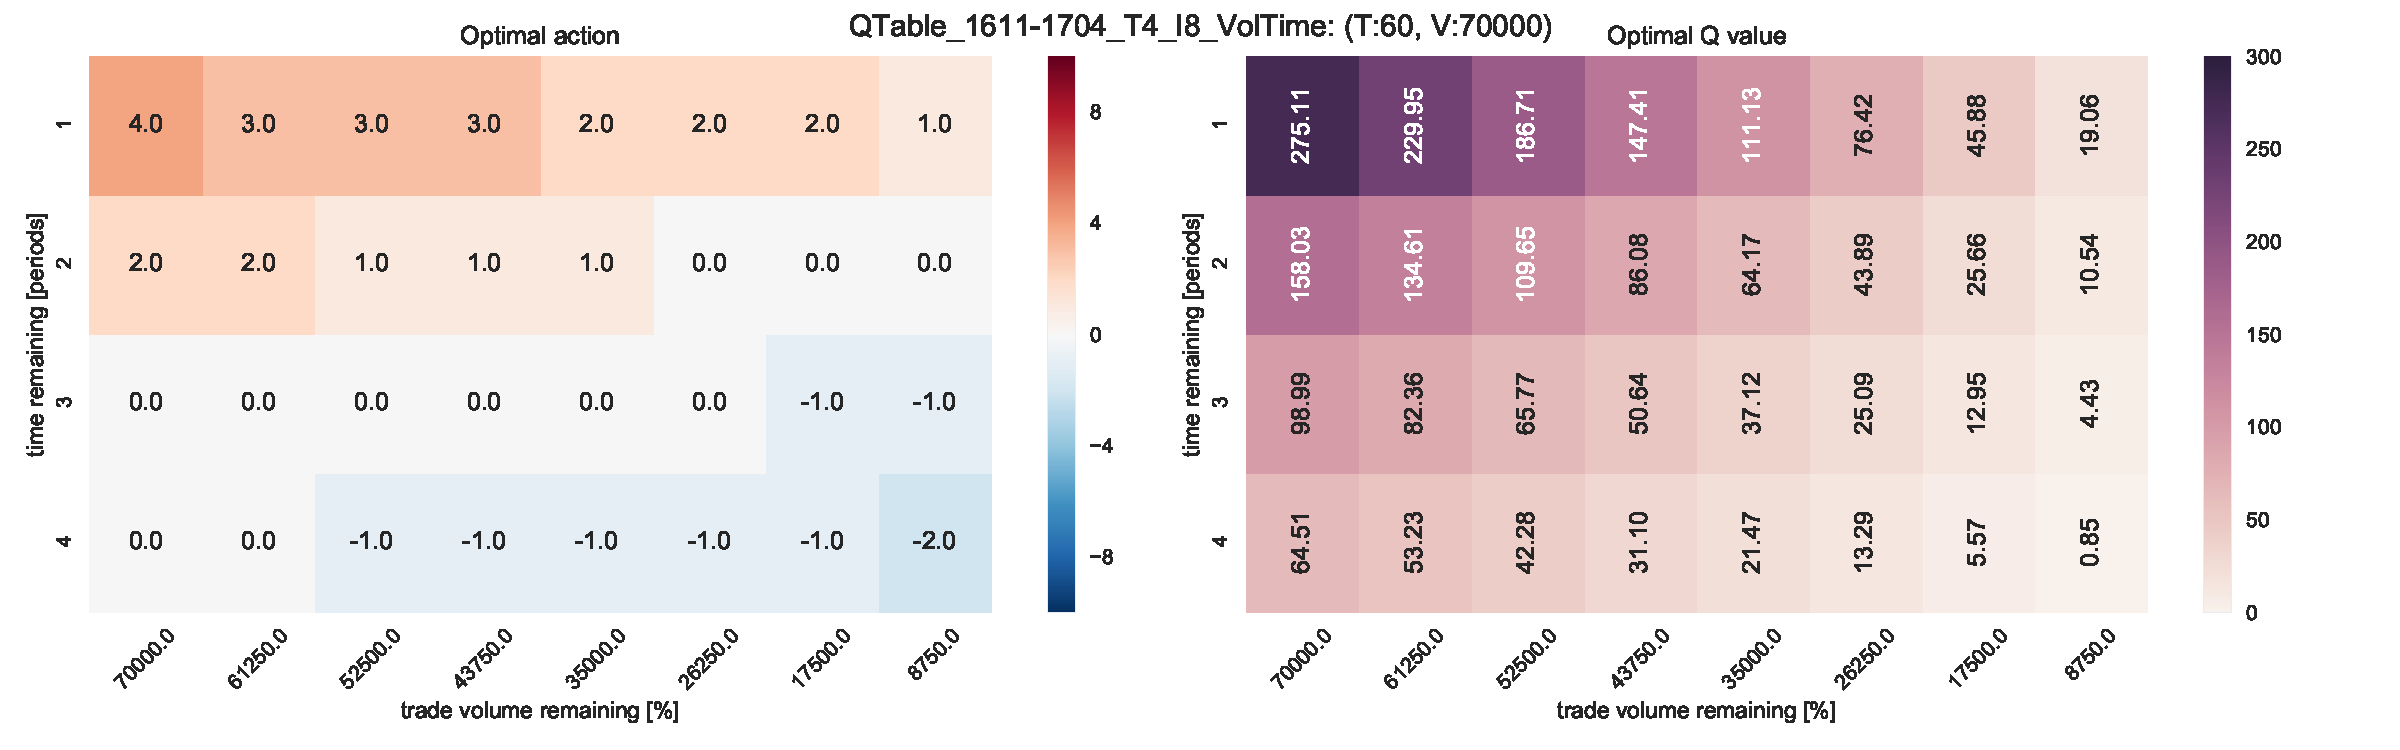
\includegraphics[width=\textwidth]{content/drawings/heatmap_VolTimeSimpre}
        		\caption{QTable of \lstinline!VolTime_simulatedTrades!-agent.}
		
    	\end{subfigure}
	
	\caption{A slight increase in aggression, if preceding trades are incorporated.}
	\label{fig:heatmap:VolTimeSimpre}
	$T=4$, $I=8$, L=15

\end{figure}

The best performing \lstinline!VolTimeSpread_disc5!-agent now undercuts costs induced by simple market orders by $-49.59\%$ (before: $-49.16\%$), the gain in comparison to the optimal \ac{SL} strategy enlarged to $-9.70\%$ (before: $-8.93\%$).\\

\subsection{Estimating Action Effects}
\label{chap:eval:additionalMarketVariables:actioneffects}

\Cref{tab:eval:additionalMarketVariables:_a_} evaluates the impact of adding (lower bound) knowledge about consequences of individual actions to the state space. That way, \lstinline!_a_4_! quotes the minimum volume immediately obtainable by a limit order placed $+0.4\%$ above the current ask price.\\

Potentially due to coarse discretization, these variables cause no major impact. Almost all \lstinline!_a*_!-agents perform worse than the underlying \lstinline!VolTime_simulatedTrades!-agent.

\begin{table}[ht]
	\centering
	\scalebox{0.6}{
	\rowcolors{1}{}{black!5}
\begin{tabular}{|lRRR|RRRR|}
\toprule
{} &  \text{slippage} &     \text{med} &     \text{std} &   \text{perf\_2} &   \text{perf\_4} &   \text{perf\_M} & \text{perf\_VolTime} \\
\midrule
\_a\_-4\_disc5 &    149.84 &   40.54 &  368.50 &  -3.27\% &  -15.04\% &  -46.00\% &       -0.52\% \\
\_a\_-3\_disc5 &    150.70 &   37.95 &  372.15 &  -2.71\% &  -14.55\% &  -45.69\% &        +0.05\% \\
\_a\_0\_disc5  &    153.01 &   45.17 &  375.98 &  -1.22\% &  -13.25\% &  -44.86\% &        +1.58\% \\
\_a\_1\_disc5  &    148.56 &   41.60 &  385.79 &  -4.10\% &  -15.77\% &  -46.46\% &       -1.37\% \\
\_a\_2\_disc5  &    149.47 &   43.47 &  368.49 &  -3.50\% &  -15.25\% &  -46.13\% &       -0.77\% \\
\_a\_3\_disc5  &    145.04 &   42.42 &  365.27 &  -6.37\% &  -17.76\% &  -47.73\% &       -3.71\% \\
\_a\_4\_disc5  &    155.52 &   40.84 &  373.98 &   +0.40\% &  -11.82\% &  -43.95\% &        +3.25\% \\
\_a\_5\_disc5  &    152.05 &   38.53 &  372.03 &  -1.84\% &  -13.79\% &  -45.21\% &        +0.94\% \\
\_a\_6\_disc5  &    151.80 &   40.39 &  371.41 &  -2.00\% &  -13.93\% &  -45.29\% &        +0.78\% \\
\_a\_7\_disc5  &    148.61 &   40.39 &  363.67 &  -4.06\% &  -15.74\% &  -46.44\% &       -1.34\% \\
\_a\_8\_disc5  &    152.46 &   41.26 &  363.02 &  -1.57\% &  -13.56\% &  -45.06\% &        +1.22\% \\
\_a\_9\_disc5  &    151.59 &   40.84 &  363.68 &  -2.14\% &  -14.05\% &  -45.37\% &        +0.64\% \\
\_a\_10\_disc5 &    150.28 &   40.84 &  363.70 &  -2.99\% &  -14.80\% &  -45.84\% &       -0.23\% \\
\midrule
VolTime\_simulatedTrades &    147.86 &   42.10 &  346.17 &   -4.55\% &  -16.17\% &  -46.72\% &       -1.84\% \\
VolTime     &    150.63 &   33.83 &  358.66 &  -2.76\% &  -14.60\% &  -45.72\% &        0.00\% \\
2           &    154.90 &   68.62 &  389.15 &   0.00\% &  -12.17\% &  -44.18\% &        +2.84\% \\
4           &    176.37 &  141.66 &  273.58 &  +13.86\% &    0.00\% &  -36.44\% &       +17.09\% \\
MarketOrder &    277.49 &  246.48 &  158.66 &  +79.14\% &   +57.33\% &    0.00\% &       +84.22\% \\
\bottomrule
\end{tabular}
}  		 
        		\caption{Evaluating the impact of action-consequence knowledge.}
		\small Average performance over the test period may 2017, currency pair USDT/BTC.\\
		
		\label{tab:eval:additionalMarketVariables:_a_}
\end{table}



\subsection{Function Approximation: BatchTree}
\label{chap:experiment:functionApprox}
In the next step the look-up table is replaced by an approximation thereof. This eliminates any need for discretization, avoids the cost scaling problem and as such, potentially helps to exploit the underlying sample transitions better. Various \ac{BT}-Agents are trained on the sample transitions collected by the improved backward collection process (see \Cref{chap:exp:simulatedTrades}). Results are shown in \Cref{tab:eval:BatchTree:simPreTrades}.\\

\begin{table}[ht]
	\centering
	\scalebox{0.6}{
\rowcolors{1}{}{black!5}
\begin{tabular}{|lRRR|RRRR|}
\toprule
{} &  \text{slippage} &     \text{med} &     \text{std} &   \text{perf\_2} &   \text{perf\_4} &   \text{perf\_M} & \text{perf\_VolTime} \\
\midrule
BT\_VolTime\_a4\_   &    163.21 &   25.48 &  466.45 &   +5.36\% &   -7.46\% &  -41.18\% &        +8.35\% \\
\cellcolor{green!25}BT\_VolTime\_a*\_       &    \cellcolor{green!25}143.24 &   38.53 &  373.35 &  \cellcolor{green!25}-7.53\% &  -18.78\% &  -48.38\% &       -4.90\% \\
BT\_VolTime &    151.08 &   47.39 &  391.02 &  \cellcolor{black!20}-2.47\% &  -14.34\% &  -45.55\% &        +0.30\% \\
\cellcolor{red!25}BT\_VolTimeSpread &    \cellcolor{red!25}249.07 &  237.29 &  142.11 & \cellcolor{red!25}+60.79\% &   +41.22\% &  -10.24\% &       +65.36\% \\
\midrule
VolTime\_simulatedTrades &    147.86 &   42.10 &  346.17 &   \cellcolor{black!20}-4.55\% &  -16.17\% &  -46.72\% &       -1.84\% \\
VolTime          &    150.63 &   33.83 &  358.66 &  -2.76\% &  -14.60\% &  -45.72\% &        0.00\% \\
2                &    154.90 &   68.62 &  389.15 &   0.00\% &  -12.17\% &  -44.18\% &        +2.84\% \\
4                &    176.37 &  141.66 &  273.58 &  +13.86\% &    0.00\% &  -36.44\% &       +17.09\% \\
MarketOrder      &    277.49 &  246.48 &  158.66 &  +79.14\% &   +57.33\% &    0.00\% &       +84.22\% \\
\bottomrule
\end{tabular}
}  		 
        		\caption{Evaluating the performance of function approximators.}
		\small Average performance over the test period may 2017, currency pair USDT/BTC.\\
		
		\label{tab:eval:BatchTree:simPreTrades}
\end{table}

While the plain \lstinline!BT_VolTime!-agent performs de facto worse than the original, discrete \lstinline!VolTime!-agent ($-2.47\%$ vs. $-4.55\%$),  agents employing individual market variables perform terribly if fed with continuous values. The worst of all, \lstinline!BT_VolTimeSpread!-agent,  performs $+60.79\%$ worse than the optimal \ac{SL} strategy!\\

Conversely, a \ac{BT}-agent trained on all fifteen \lstinline!_a*_effects!-variables simultaneously lifts the \ac{BT} performance from $-2.47\%$ to $-7.53\%$, which is a good result. Unfortunately, it does not catch up with the previously attained $-9.7\%$ (see \Cref{chap:exp:simulatedTrades}).\\


\Cref{fig:heatmap:BatchTree:SimPreTrades} shows exemplary for the plain \lstinline!VolTime!-agent, how the \ac{BT}-agent is able to deliver a more accurate resolution of q-values and optimal actions.

\begin{figure}[ht]
	\centering	
	\begin{subfigure}[b]{0.8\textwidth}
        		\centering
        		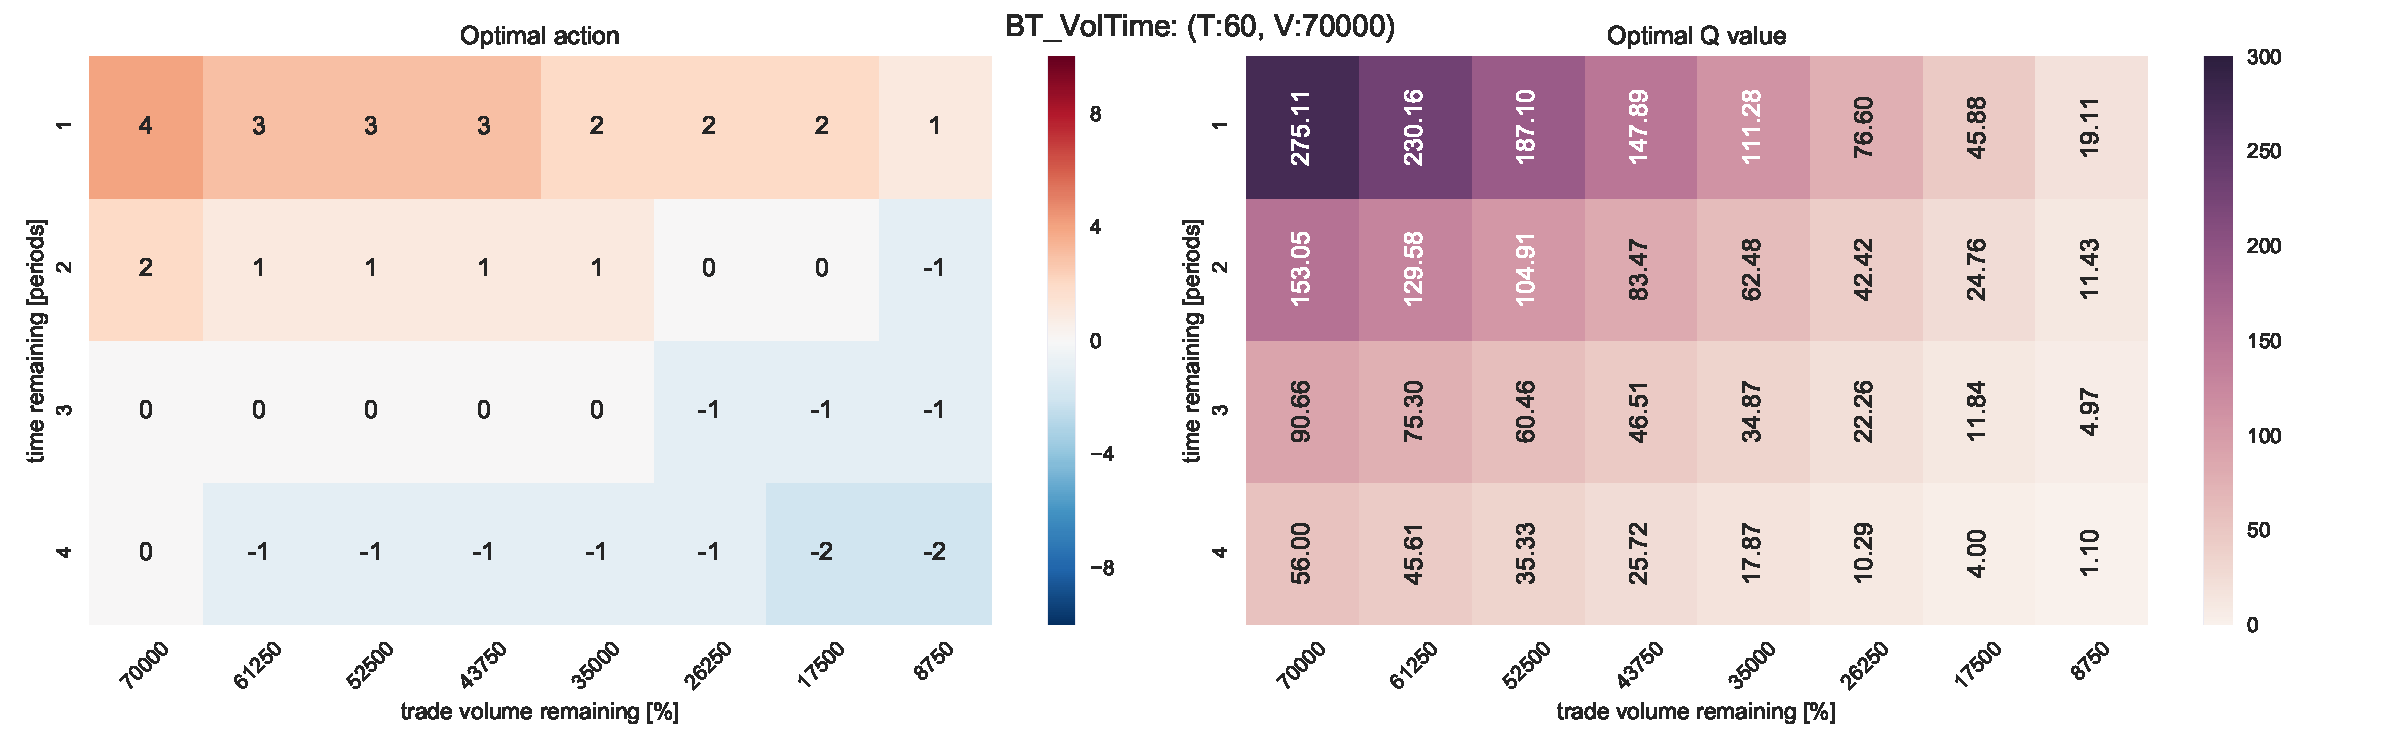
\includegraphics[width=\textwidth]{content/drawings/BT_VolTime_3_vol08}
        		\caption{QTable by \lstinline!VolTime!-agent.}
    	\end{subfigure}
	\begin{subfigure}[b]{0.8\textwidth}
        		\centering
        		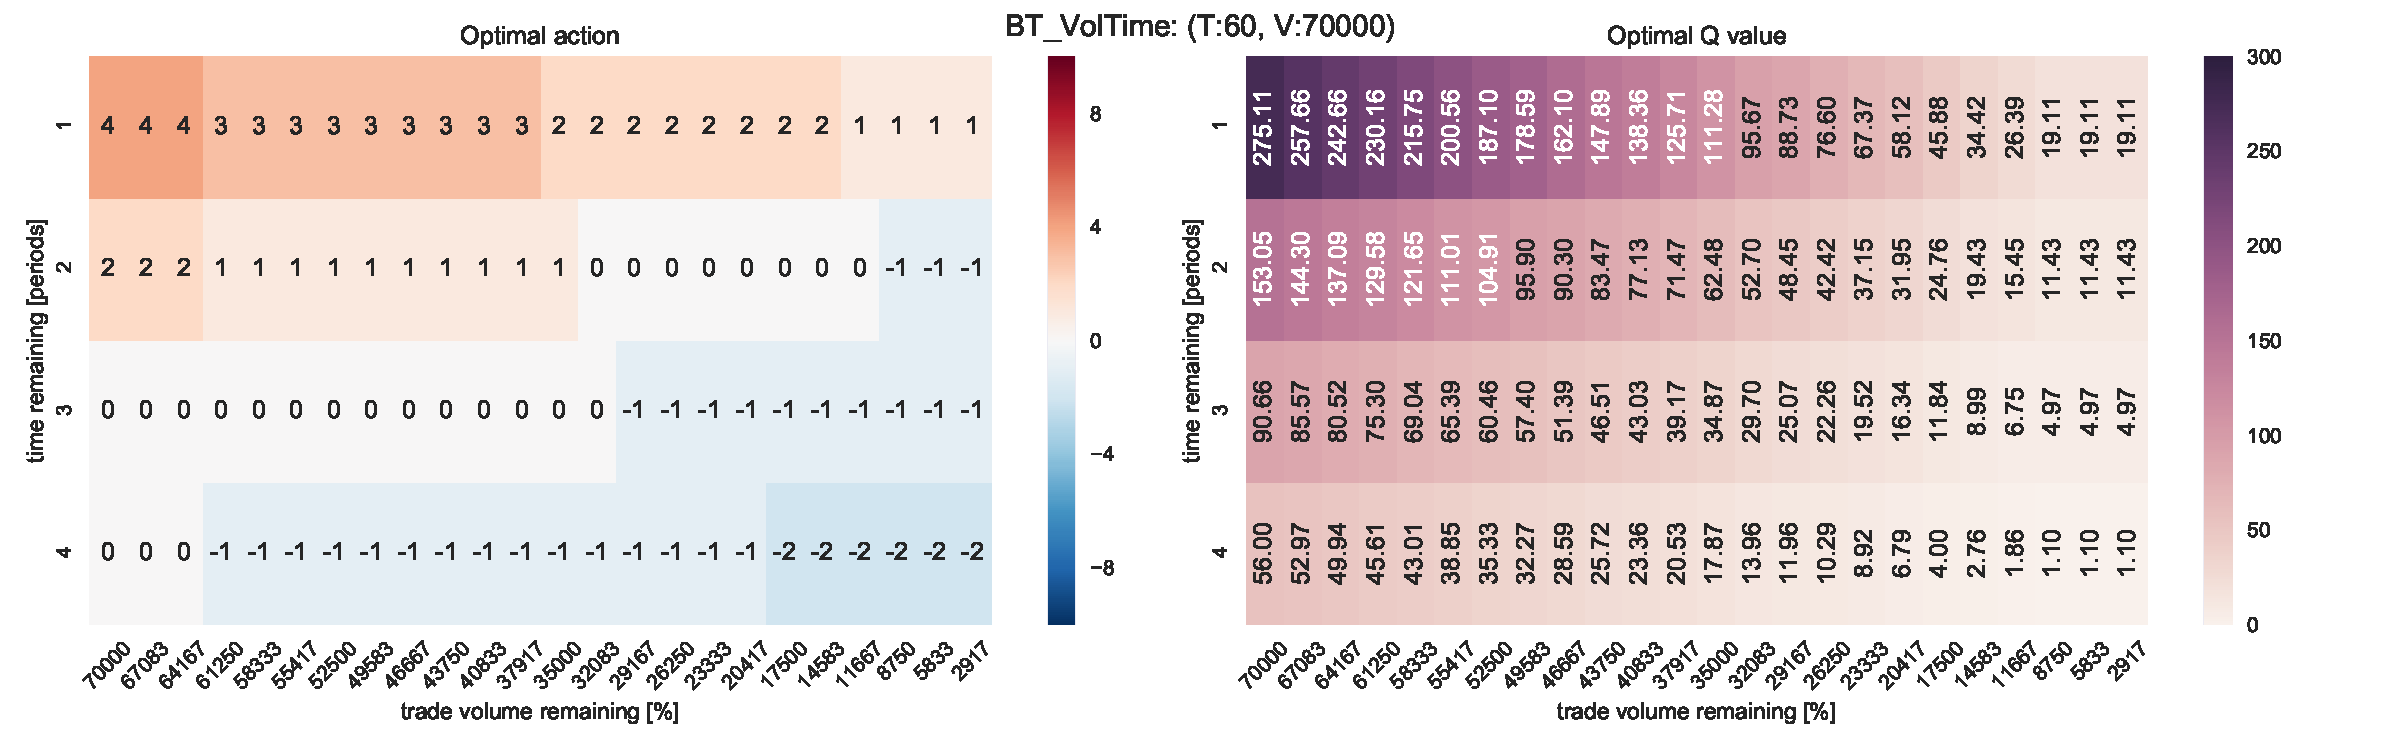
\includegraphics[width=\textwidth]{content/drawings/BT_VolTime_3_vol24}
        		\caption{QTable approximation by \lstinline!BT_VolTime!-agent (High resolution).}
		
    	\end{subfigure}
	
	\caption{The \ac{BT}-agent generalizes to continuous states.}
	\label{fig:heatmap:BatchTree:SimPreTrades}

\end{figure}









\section{Forward Learning Experiments}
\label{chap:experiments:forward}
Based on the same training data and simulator settings as used in the preceding Backward Learning Experiments, the novel forward sampling approach (see \Cref{chap:forwardlearning}) is examined.\\

The \lstinline!BT_Forward!-agent samples from the previously shuffled training data, following an $\epsilon$-greedy strategy. In each exploration phase the respective orderbook window is run through up to 60 times, while only disparate paths are traced. After every 256 exploration phases, the underlying RandomForestRegressor is retrained from scratch, using all transition samples collected to this point. Intermediate models are stored, to document the learning progress over time. The continuous state space consists of both private variables and the fifteen action-effect-variables \lstinline!_a*_!, as introduced in \Cref{chap:exp:additionalmarketvars}.\\

The performance of all sixteen intermediate models is shown in \Cref{tab:eval:ForwardSampling:BT}. Starting vaguely halfway through the training data, the \lstinline!BT_Forward!-agent outperforms all previously examined agents, before the final model constitutes the overall winner with an improvement of $-11.41\%$ over the optimal \ac{SL} strategy.\\

\begin{table}[h!]
	\centering
	\scalebox{0.6}{
\rowcolors{1}{}{black!5}
\begin{tabular}{|lRRR|RRRR|}
\toprule
{} &  \text{slippage} &     \text{med} &     \text{std} &   \text{perf\_2} &   \text{perf\_4} &   \text{perf\_M} & \text{perf\_VolTime} \\
\midrule
BT\_Forward\_samples\_025.078  &    143.72 &   74.69 &  300.93 &   -7.22\% &  -18.52\% &  -48.21\% &       -4.59\% \\
BT\_Forward\_samples\_043.334  &    147.92 &   82.24 &  310.49 &   -4.51\% &  -16.13\% &  -46.69\% &       -1.80\% \\
BT\_Forward\_samples\_061.103  &    149.56 &   77.33 &  288.56 &   -3.45\% &  -15.20\% &  -46.10\% &       -0.71\% \\
BT\_Forward\_samples\_079.809  &    146.67 &   77.20 &  277.43 &   -5.31\% &  -16.84\% &  -47.14\% &       -2.62\% \\
BT\_Forward\_samples\_097.615  &    143.45 &   73.18 &  281.71 &   -7.40\% &  -18.67\% &  -48.31\% &       -4.77\% \\
BT\_Forward\_samples\_116.008 &    144.26 &   77.94 &  285.80 &   -6.87\% &  -18.21\% &  -48.01\% &       -4.23\% \\
BT\_Forward\_samples\_134.011 &    138.22 &   73.30 &  269.71 &  -10.77\% &  -21.63\% &  -50.19\% &       -8.24\% \\
BT\_Forward\_samples\_152.352 &    136.90 &   69.59 &  264.95 &  -11.62\% &  -22.38\% &  -50.66\% &       -9.11\% \\
BT\_Forward\_samples\_170.605 &    137.75 &   77.50 &  261.17 &  -11.07\% &  -21.90\% &  -50.36\% &       -8.55\% \\
BT\_Forward\_samples\_188.224 &    137.64 &   73.71 &  253.37 &  -11.14\% &  -21.96\% &  -50.40\% &       -8.62\% \\
BT\_Forward\_samples\_206.409 &    137.10 &   74.22 &  257.54 &  -11.49\% &  -22.27\% &  -50.59\% &       -8.98\% \\
BT\_Forward\_samples\_224.083 &    142.90 &   75.43 &  265.78 &   -7.75\% &  -18.98\% &  -48.50\% &       -5.13\% \\
BT\_Forward\_samples\_242.342 &    129.85 &   74.43 &  239.96 &  -16.17\% &  -26.37\% &  -53.20\% &      -13.79\% \\
BT\_Forward\_samples\_261.018 &    137.98 &   75.69 &  248.07 &  -10.92\% &  -21.77\% &  -50.27\% &       -8.39\% \\
BT\_Forward\_samples\_279.347 &    138.79 &   75.28 &  258.49 &  -10.40\% &  -21.31\% &  -49.98\% &       -7.86\% \\
BT\_Forward\_samples\_298.020 &    \cellcolor{green!25}137.23 &   \cellcolor{green!25}78.71 &  \cellcolor{green!25}242.88 &  \cellcolor{green!25}-11.41\% &  \cellcolor{green!25}-22.19\% &  \cellcolor{green!25}-50.55\% &       \cellcolor{green!25}-8.89\% \\
\midrule
VolTime                        &    150.63 &   33.83 &  358.66 &   -2.76\% &  -14.60\% &  -45.72\% &        0.00\% \\
2                              &    154.90 &   68.62 &  389.15 &    0.00\% &  -12.17\% &  -44.18\% &        +2.84\% \\
4                              &    176.37 &  141.66 &  273.58 &   +13.86\% &    0.00\% &  -36.44\% &       +17.09\% \\
MarketOrder                    &    277.49 &  246.48 &  158.66 &   +79.14\% &   +57.33\% &    0.00\% &       +84.22\% \\
\bottomrule
\end{tabular}
}  		 
        		\caption{Performance growth of the final \lstinline!BT_Forward!-agent.}
		\small Average performance over the test period may 2017, currency pair USDT/BTC.\\
		
		\label{tab:eval:ForwardSampling:BT}
\end{table}

\Cref{fig:BTForward:performance} visualized the \lstinline!BT_Forward!-agents performance evolution over the training phase. The horizontal lines refer to baselines and previously achieved performances.\\

\begin{figure}[h!]
	\centering
	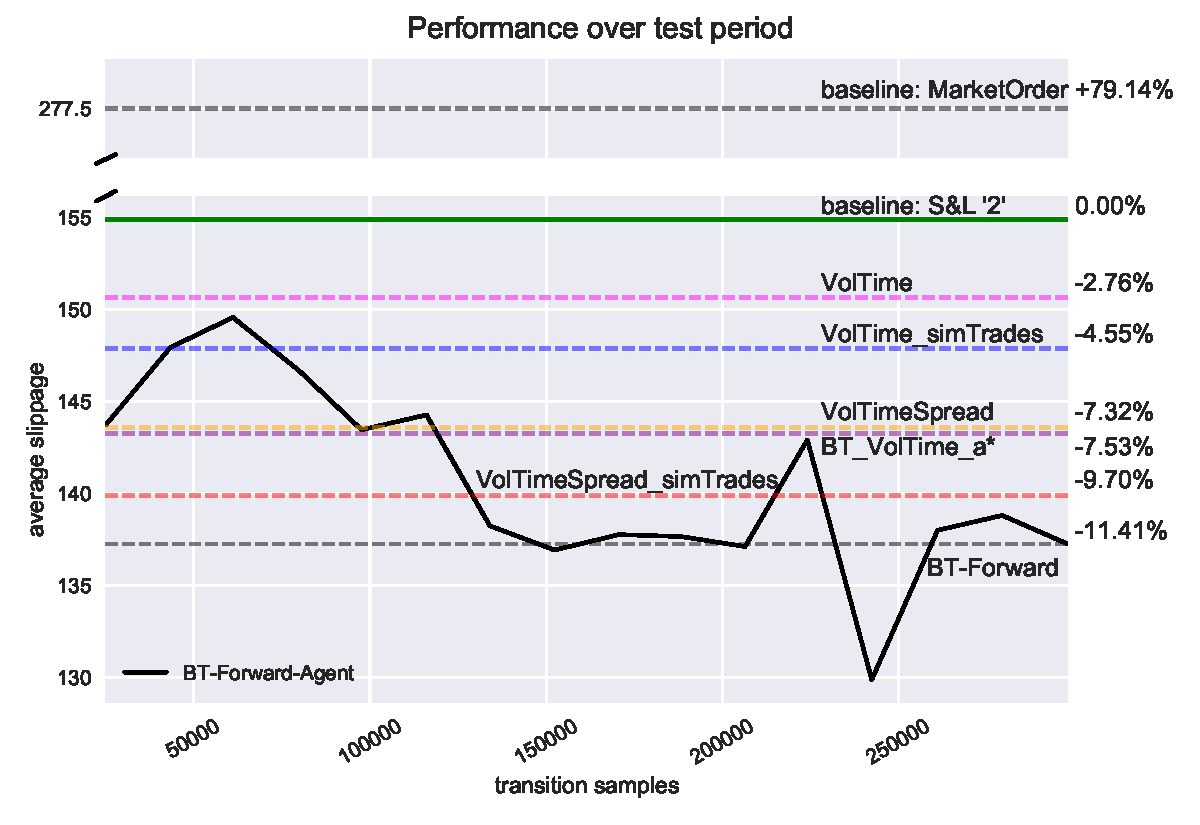
\includegraphics[width=0.8\textwidth]{content/drawings/BT_Forward_Performance}
	\caption{The \lstinline!BT_Forward!-agent performance on the test period.}
	\label{fig:BTForward:performance}

\end{figure}











\cleardoublepage{}